\documentclass[12pt]{article}
\usepackage{amsmath}
\usepackage{amssymb}
\usepackage{color}
\usepackage{tikz}

\begin{document}

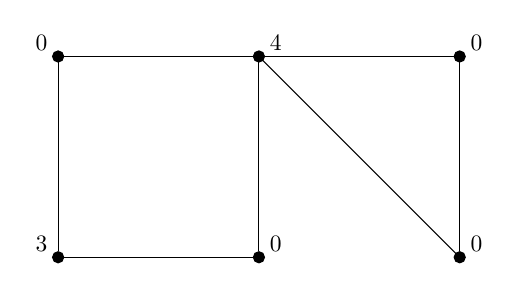
\begin{tikzpicture}[scale=.85, transform shape]

%% 3-regular graph with 10 vertices

\node [draw, shape=circle,fill=black,scale=0.5] (u0) at  (3,2) {};
\node [draw, shape=circle,fill=black,scale=0.5] (u1) at  (3,5) {};
\node [draw, shape=circle,fill=black,scale=0.5] (u2) at  (6,5) {};
\node [draw, shape=circle,fill=black,scale=0.5] (u3) at  (6,2) {};
\node [draw, shape=circle,fill=black,scale=0.5] (u4) at  (9,5) {};
\node [draw, shape=circle,fill=black,scale=0.5] (u5) at  (9,2) {};
\draw (u0)--(u1);
\draw (u1)--(u2);
\draw (u2)--(u3);
\draw (u3)--(u0);
\draw (u2)--(u4);
\draw (u4)--(u5);
\draw (u2)--(u5);
\node[draw=none, fill=none] at (2.75,2.2){ $3$};
\node[draw=none, fill=none] at (6.25,2.2){ $0$};
\node[draw=none, fill=none] at (2.75,5.2){ $0$};
\node[draw=none, fill=none] at (6.25,5.2){ $4$};
\node[draw=none, fill=none] at (9.25,2.2){ $0$};
\node[draw=none, fill=none] at (9.25,5.2){ $0$};

%%
\end{tikzpicture}

\end{document}